\documentclass[tikz,border=8pt]{standalone}
% Shared look for every TikZ diagram. Load with \input{../../tools/tikz-style.tex}
\usepackage[T1]{fontenc}
\usepackage{lmodern}
\renewcommand{\sfdefault}{lmr}  % diagrams use the same serif as the text
\usetikzlibrary{arrows.meta, positioning, shapes.geometric, calc, fit, backgrounds}
\definecolor{cblue}{HTML}{4C78A8}
\definecolor{corange}{HTML}{F58518}
\definecolor{cgreen}{HTML}{54A24B}
\definecolor{cred}{HTML}{E45756}
\definecolor{cpurple}{HTML}{B279A2}
\definecolor{cgrey}{HTML}{6B6B6B}
\tikzset{
  every picture/.style={font=\sffamily, line width=1.2pt},
  box/.style={draw=#1, fill=#1!12, rounded corners=4pt, align=center, inner sep=7pt, minimum height=1.1cm},
  box/.default=cgrey,
  arrow/.style={-{Stealth[length=3mm]}, draw=cgrey, line width=1.4pt},
  title/.style={font=\sffamily\bfseries\Large},
  note/.style={font=\sffamily\small, text=cgrey, align=center},
}
\AtBeginDocument{\hyphenpenalty=10000 \exhyphenpenalty=10000}

\begin{document}
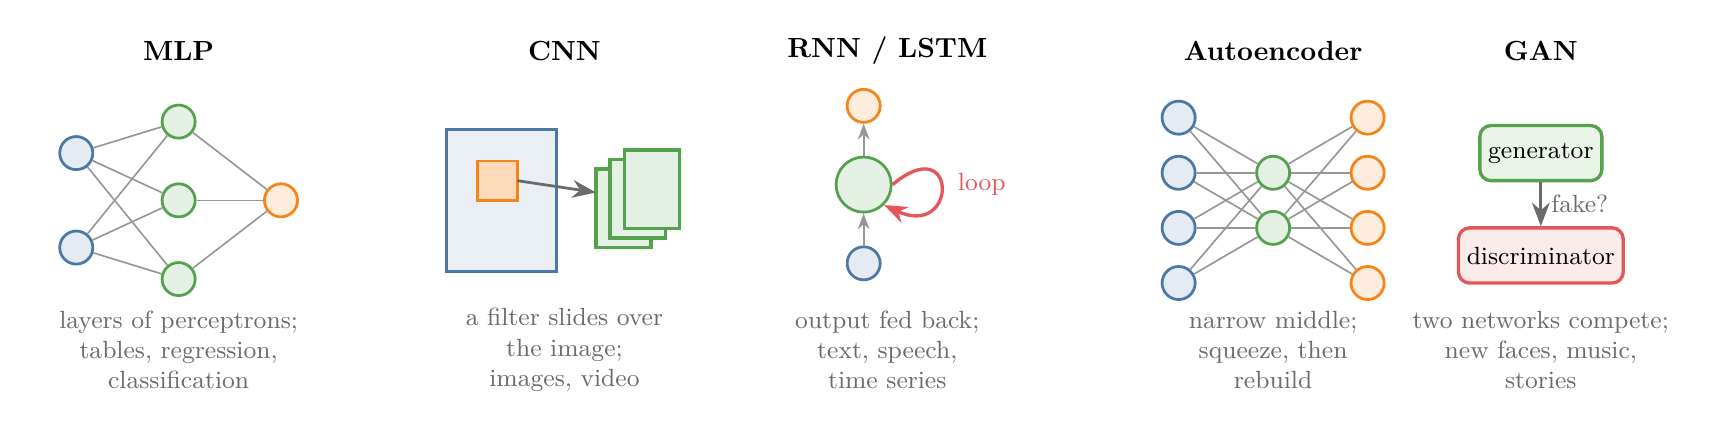
\begin{tikzpicture}[n/.style={circle, draw=#1, fill=#1!15, minimum size=0.42cm, inner sep=0pt, line width=1pt}, e/.style={draw=cgrey!70, line width=0.6pt}, lab/.style={font=\sffamily\bfseries}, sub/.style={note, text width=3.6cm}]
% MLP
\begin{scope}[shift={(0,0)}]
  \foreach \y [count=\i] in {0.6,-0.6} \node[n=cblue] (a\i) at (0,\y) {};
  \foreach \y [count=\i] in {1.0,0,-1.0} \node[n=cgreen] (b\i) at (1.3,\y) {};
  \node[n=corange] (c) at (2.6,0) {};
  \foreach \i in {1,2} \foreach \j in {1,2,3} \draw[e] (a\i)--(b\j);
  \foreach \j in {1,2,3} \draw[e] (b\j)--(c);
  \node[lab] at (1.3,1.9) {MLP};
  \node[sub] at (1.3,-1.9) {layers of perceptrons;\\tables, regression,\\classification};
\end{scope}
% CNN
\begin{scope}[shift={(5,0)}]
  \draw[draw=cblue, fill=cblue!12] (-0.3,-0.9) rectangle (1.1,0.9);
  \draw[draw=corange, fill=corange!30, line width=1pt] (0.1,0.0) rectangle (0.6,0.5);
  \foreach \k in {0,1,2} \draw[draw=cgreen, fill=cgreen!15] (1.6+0.18*\k,-0.6+0.12*\k) rectangle (2.3+0.18*\k,0.4+0.12*\k);
  \draw[arrow, line width=1pt] (0.6,0.25) -- (1.6,0.1);
  \node[lab] at (1.2,1.9) {CNN};
  \node[sub] at (1.2,-1.9) {a filter slides over\\the image;\\images, video};
\end{scope}
% RNN
\begin{scope}[shift={(10,0)}]
  \node[n=cblue] (x) at (0,-0.8) {};
  \node[n=cgreen, minimum size=0.7cm] (h) at (0,0.2) {};
  \node[n=corange] (y) at (0,1.2) {};
  \draw[e, -{Stealth}] (x)--(h); \draw[e, -{Stealth}] (h)--(y);
  \draw[cred, line width=1.2pt, -{Stealth}] (h.east) .. controls (1.2,0.9) and (1.2,-0.5) .. (h.south east);
  \node[note, text=cred] at (1.5,0.2) {loop};
  \node[lab] at (0.3,1.9) {RNN / LSTM};
  \node[sub] at (0.3,-1.9) {output fed back;\\text, speech,\\time series};
\end{scope}
% Autoencoder
\begin{scope}[shift={(14,0)}]
  \foreach \y [count=\i] in {1.05,0.35,-0.35,-1.05} \node[n=cblue] (p\i) at (0,\y) {};
  \foreach \y [count=\i] in {0.35,-0.35} \node[n=cgreen] (q\i) at (1.2,\y) {};
  \foreach \y [count=\i] in {1.05,0.35,-0.35,-1.05} \node[n=corange] (r\i) at (2.4,\y) {};
  \foreach \i in {1,...,4} \foreach \j in {1,2} {\draw[e] (p\i)--(q\j); \draw[e] (q\j)--(r\i);}
  \node[lab] at (1.2,1.9) {Autoencoder};
  \node[sub] at (1.2,-1.9) {narrow middle;\\squeeze, then\\rebuild};
\end{scope}
% GAN
\begin{scope}[shift={(18.6,0)}]
  \node[box=cgreen, minimum height=0.7cm, inner sep=3pt, font=\sffamily\small] (g) at (0,0.6) {generator};
  \node[box=cred, minimum height=0.7cm, inner sep=3pt, font=\sffamily\small] (d) at (0,-0.7) {discriminator};
  \draw[arrow, line width=1pt] (g) -- node[right, note] {fake?} (d);
  \node[lab] at (0,1.9) {GAN};
  \node[sub] at (0,-1.9) {two networks compete;\\new faces, music,\\stories};
\end{scope}
\end{tikzpicture}
\end{document}
